\documentclass[11pt]{article}

    \usepackage[breakable]{tcolorbox}
    \usepackage{parskip} % Stop auto-indenting (to mimic markdown behaviour)
    

    % Basic figure setup, for now with no caption control since it's done
    % automatically by Pandoc (which extracts ![](path) syntax from Markdown).
    \usepackage{graphicx}
    % Maintain compatibility with old templates. Remove in nbconvert 6.0
    \let\Oldincludegraphics\includegraphics
    % Ensure that by default, figures have no caption (until we provide a
    % proper Figure object with a Caption API and a way to capture that
    % in the conversion process - todo).
    \usepackage{caption}
    \DeclareCaptionFormat{nocaption}{}
    \captionsetup{format=nocaption,aboveskip=0pt,belowskip=0pt}

    \usepackage{float}
    \floatplacement{figure}{H} % forces figures to be placed at the correct location
    \usepackage{xcolor} % Allow colors to be defined
    \usepackage{enumerate} % Needed for markdown enumerations to work
    \usepackage{geometry} % Used to adjust the document margins
    \usepackage{amsmath} % Equations
    \usepackage{amssymb} % Equations
    \usepackage{textcomp} % defines textquotesingle
    % Hack from http://tex.stackexchange.com/a/47451/13684:
    \AtBeginDocument{%
        \def\PYZsq{\textquotesingle}% Upright quotes in Pygmentized code
    }
    \usepackage{upquote} % Upright quotes for verbatim code
    \usepackage{eurosym} % defines \euro

    \usepackage{iftex}
    \ifPDFTeX
        \usepackage[T1]{fontenc}
        \IfFileExists{alphabeta.sty}{
              \usepackage{alphabeta}
          }{
              \usepackage[mathletters]{ucs}
              \usepackage[utf8x]{inputenc}
          }
    \else
        \usepackage{fontspec}
        \usepackage{unicode-math}
    \fi

    \usepackage{fancyvrb} % verbatim replacement that allows latex
    \usepackage{grffile} % extends the file name processing of package graphics
                         % to support a larger range
    \makeatletter % fix for old versions of grffile with XeLaTeX
    \@ifpackagelater{grffile}{2019/11/01}
    {
      % Do nothing on new versions
    }
    {
      \def\Gread@@xetex#1{%
        \IfFileExists{"\Gin@base".bb}%
        {\Gread@eps{\Gin@base.bb}}%
        {\Gread@@xetex@aux#1}%
      }
    }
    \makeatother
    \usepackage[Export]{adjustbox} % Used to constrain images to a maximum size
    \adjustboxset{max size={0.9\linewidth}{0.9\paperheight}}

    % The hyperref package gives us a pdf with properly built
    % internal navigation ('pdf bookmarks' for the table of contents,
    % internal cross-reference links, web links for URLs, etc.)
    \usepackage{hyperref}
    % The default LaTeX title has an obnoxious amount of whitespace. By default,
    % titling removes some of it. It also provides customization options.
    \usepackage{titling}
    \usepackage{longtable} % longtable support required by pandoc >1.10
    \usepackage{booktabs}  % table support for pandoc > 1.12.2
    \usepackage{array}     % table support for pandoc >= 2.11.3
    \usepackage{calc}      % table minipage width calculation for pandoc >= 2.11.1
    \usepackage[inline]{enumitem} % IRkernel/repr support (it uses the enumerate* environment)
    \usepackage[normalem]{ulem} % ulem is needed to support strikethroughs (\sout)
                                % normalem makes italics be italics, not underlines
    \usepackage{soul}      % strikethrough (\st) support for pandoc >= 3.0.0
    \usepackage{mathrsfs}
    

    
    % Colors for the hyperref package
    \definecolor{urlcolor}{rgb}{0,.145,.698}
    \definecolor{linkcolor}{rgb}{.71,0.21,0.01}
    \definecolor{citecolor}{rgb}{.12,.54,.11}

    % ANSI colors
    \definecolor{ansi-black}{HTML}{3E424D}
    \definecolor{ansi-black-intense}{HTML}{282C36}
    \definecolor{ansi-red}{HTML}{E75C58}
    \definecolor{ansi-red-intense}{HTML}{B22B31}
    \definecolor{ansi-green}{HTML}{00A250}
    \definecolor{ansi-green-intense}{HTML}{007427}
    \definecolor{ansi-yellow}{HTML}{DDB62B}
    \definecolor{ansi-yellow-intense}{HTML}{B27D12}
    \definecolor{ansi-blue}{HTML}{208FFB}
    \definecolor{ansi-blue-intense}{HTML}{0065CA}
    \definecolor{ansi-magenta}{HTML}{D160C4}
    \definecolor{ansi-magenta-intense}{HTML}{A03196}
    \definecolor{ansi-cyan}{HTML}{60C6C8}
    \definecolor{ansi-cyan-intense}{HTML}{258F8F}
    \definecolor{ansi-white}{HTML}{C5C1B4}
    \definecolor{ansi-white-intense}{HTML}{A1A6B2}
    \definecolor{ansi-default-inverse-fg}{HTML}{FFFFFF}
    \definecolor{ansi-default-inverse-bg}{HTML}{000000}

    % common color for the border for error outputs.
    \definecolor{outerrorbackground}{HTML}{FFDFDF}

    % commands and environments needed by pandoc snippets
    % extracted from the output of `pandoc -s`
    \providecommand{\tightlist}{%
      \setlength{\itemsep}{0pt}\setlength{\parskip}{0pt}}
    \DefineVerbatimEnvironment{Highlighting}{Verbatim}{commandchars=\\\{\}}
    % Add ',fontsize=\small' for more characters per line
    \newenvironment{Shaded}{}{}
    \newcommand{\KeywordTok}[1]{\textcolor[rgb]{0.00,0.44,0.13}{\textbf{{#1}}}}
    \newcommand{\DataTypeTok}[1]{\textcolor[rgb]{0.56,0.13,0.00}{{#1}}}
    \newcommand{\DecValTok}[1]{\textcolor[rgb]{0.25,0.63,0.44}{{#1}}}
    \newcommand{\BaseNTok}[1]{\textcolor[rgb]{0.25,0.63,0.44}{{#1}}}
    \newcommand{\FloatTok}[1]{\textcolor[rgb]{0.25,0.63,0.44}{{#1}}}
    \newcommand{\CharTok}[1]{\textcolor[rgb]{0.25,0.44,0.63}{{#1}}}
    \newcommand{\StringTok}[1]{\textcolor[rgb]{0.25,0.44,0.63}{{#1}}}
    \newcommand{\CommentTok}[1]{\textcolor[rgb]{0.38,0.63,0.69}{\textit{{#1}}}}
    \newcommand{\OtherTok}[1]{\textcolor[rgb]{0.00,0.44,0.13}{{#1}}}
    \newcommand{\AlertTok}[1]{\textcolor[rgb]{1.00,0.00,0.00}{\textbf{{#1}}}}
    \newcommand{\FunctionTok}[1]{\textcolor[rgb]{0.02,0.16,0.49}{{#1}}}
    \newcommand{\RegionMarkerTok}[1]{{#1}}
    \newcommand{\ErrorTok}[1]{\textcolor[rgb]{1.00,0.00,0.00}{\textbf{{#1}}}}
    \newcommand{\NormalTok}[1]{{#1}}

    % Additional commands for more recent versions of Pandoc
    \newcommand{\ConstantTok}[1]{\textcolor[rgb]{0.53,0.00,0.00}{{#1}}}
    \newcommand{\SpecialCharTok}[1]{\textcolor[rgb]{0.25,0.44,0.63}{{#1}}}
    \newcommand{\VerbatimStringTok}[1]{\textcolor[rgb]{0.25,0.44,0.63}{{#1}}}
    \newcommand{\SpecialStringTok}[1]{\textcolor[rgb]{0.73,0.40,0.53}{{#1}}}
    \newcommand{\ImportTok}[1]{{#1}}
    \newcommand{\DocumentationTok}[1]{\textcolor[rgb]{0.73,0.13,0.13}{\textit{{#1}}}}
    \newcommand{\AnnotationTok}[1]{\textcolor[rgb]{0.38,0.63,0.69}{\textbf{\textit{{#1}}}}}
    \newcommand{\CommentVarTok}[1]{\textcolor[rgb]{0.38,0.63,0.69}{\textbf{\textit{{#1}}}}}
    \newcommand{\VariableTok}[1]{\textcolor[rgb]{0.10,0.09,0.49}{{#1}}}
    \newcommand{\ControlFlowTok}[1]{\textcolor[rgb]{0.00,0.44,0.13}{\textbf{{#1}}}}
    \newcommand{\OperatorTok}[1]{\textcolor[rgb]{0.40,0.40,0.40}{{#1}}}
    \newcommand{\BuiltInTok}[1]{{#1}}
    \newcommand{\ExtensionTok}[1]{{#1}}
    \newcommand{\PreprocessorTok}[1]{\textcolor[rgb]{0.74,0.48,0.00}{{#1}}}
    \newcommand{\AttributeTok}[1]{\textcolor[rgb]{0.49,0.56,0.16}{{#1}}}
    \newcommand{\InformationTok}[1]{\textcolor[rgb]{0.38,0.63,0.69}{\textbf{\textit{{#1}}}}}
    \newcommand{\WarningTok}[1]{\textcolor[rgb]{0.38,0.63,0.69}{\textbf{\textit{{#1}}}}}


    % Define a nice break command that doesn't care if a line doesn't already
    % exist.
    \def\br{\hspace*{\fill} \\* }
    % Math Jax compatibility definitions
    \def\gt{>}
    \def\lt{<}
    \let\Oldtex\TeX
    \let\Oldlatex\LaTeX
    \renewcommand{\TeX}{\textrm{\Oldtex}}
    \renewcommand{\LaTeX}{\textrm{\Oldlatex}}
    % Document parameters
    % Document title
    \title{report}
    
    
    
    
    
    
    
% Pygments definitions
\makeatletter
\def\PY@reset{\let\PY@it=\relax \let\PY@bf=\relax%
    \let\PY@ul=\relax \let\PY@tc=\relax%
    \let\PY@bc=\relax \let\PY@ff=\relax}
\def\PY@tok#1{\csname PY@tok@#1\endcsname}
\def\PY@toks#1+{\ifx\relax#1\empty\else%
    \PY@tok{#1}\expandafter\PY@toks\fi}
\def\PY@do#1{\PY@bc{\PY@tc{\PY@ul{%
    \PY@it{\PY@bf{\PY@ff{#1}}}}}}}
\def\PY#1#2{\PY@reset\PY@toks#1+\relax+\PY@do{#2}}

\@namedef{PY@tok@w}{\def\PY@tc##1{\textcolor[rgb]{0.73,0.73,0.73}{##1}}}
\@namedef{PY@tok@c}{\let\PY@it=\textit\def\PY@tc##1{\textcolor[rgb]{0.24,0.48,0.48}{##1}}}
\@namedef{PY@tok@cp}{\def\PY@tc##1{\textcolor[rgb]{0.61,0.40,0.00}{##1}}}
\@namedef{PY@tok@k}{\let\PY@bf=\textbf\def\PY@tc##1{\textcolor[rgb]{0.00,0.50,0.00}{##1}}}
\@namedef{PY@tok@kp}{\def\PY@tc##1{\textcolor[rgb]{0.00,0.50,0.00}{##1}}}
\@namedef{PY@tok@kt}{\def\PY@tc##1{\textcolor[rgb]{0.69,0.00,0.25}{##1}}}
\@namedef{PY@tok@o}{\def\PY@tc##1{\textcolor[rgb]{0.40,0.40,0.40}{##1}}}
\@namedef{PY@tok@ow}{\let\PY@bf=\textbf\def\PY@tc##1{\textcolor[rgb]{0.67,0.13,1.00}{##1}}}
\@namedef{PY@tok@nb}{\def\PY@tc##1{\textcolor[rgb]{0.00,0.50,0.00}{##1}}}
\@namedef{PY@tok@nf}{\def\PY@tc##1{\textcolor[rgb]{0.00,0.00,1.00}{##1}}}
\@namedef{PY@tok@nc}{\let\PY@bf=\textbf\def\PY@tc##1{\textcolor[rgb]{0.00,0.00,1.00}{##1}}}
\@namedef{PY@tok@nn}{\let\PY@bf=\textbf\def\PY@tc##1{\textcolor[rgb]{0.00,0.00,1.00}{##1}}}
\@namedef{PY@tok@ne}{\let\PY@bf=\textbf\def\PY@tc##1{\textcolor[rgb]{0.80,0.25,0.22}{##1}}}
\@namedef{PY@tok@nv}{\def\PY@tc##1{\textcolor[rgb]{0.10,0.09,0.49}{##1}}}
\@namedef{PY@tok@no}{\def\PY@tc##1{\textcolor[rgb]{0.53,0.00,0.00}{##1}}}
\@namedef{PY@tok@nl}{\def\PY@tc##1{\textcolor[rgb]{0.46,0.46,0.00}{##1}}}
\@namedef{PY@tok@ni}{\let\PY@bf=\textbf\def\PY@tc##1{\textcolor[rgb]{0.44,0.44,0.44}{##1}}}
\@namedef{PY@tok@na}{\def\PY@tc##1{\textcolor[rgb]{0.41,0.47,0.13}{##1}}}
\@namedef{PY@tok@nt}{\let\PY@bf=\textbf\def\PY@tc##1{\textcolor[rgb]{0.00,0.50,0.00}{##1}}}
\@namedef{PY@tok@nd}{\def\PY@tc##1{\textcolor[rgb]{0.67,0.13,1.00}{##1}}}
\@namedef{PY@tok@s}{\def\PY@tc##1{\textcolor[rgb]{0.73,0.13,0.13}{##1}}}
\@namedef{PY@tok@sd}{\let\PY@it=\textit\def\PY@tc##1{\textcolor[rgb]{0.73,0.13,0.13}{##1}}}
\@namedef{PY@tok@si}{\let\PY@bf=\textbf\def\PY@tc##1{\textcolor[rgb]{0.64,0.35,0.47}{##1}}}
\@namedef{PY@tok@se}{\let\PY@bf=\textbf\def\PY@tc##1{\textcolor[rgb]{0.67,0.36,0.12}{##1}}}
\@namedef{PY@tok@sr}{\def\PY@tc##1{\textcolor[rgb]{0.64,0.35,0.47}{##1}}}
\@namedef{PY@tok@ss}{\def\PY@tc##1{\textcolor[rgb]{0.10,0.09,0.49}{##1}}}
\@namedef{PY@tok@sx}{\def\PY@tc##1{\textcolor[rgb]{0.00,0.50,0.00}{##1}}}
\@namedef{PY@tok@m}{\def\PY@tc##1{\textcolor[rgb]{0.40,0.40,0.40}{##1}}}
\@namedef{PY@tok@gh}{\let\PY@bf=\textbf\def\PY@tc##1{\textcolor[rgb]{0.00,0.00,0.50}{##1}}}
\@namedef{PY@tok@gu}{\let\PY@bf=\textbf\def\PY@tc##1{\textcolor[rgb]{0.50,0.00,0.50}{##1}}}
\@namedef{PY@tok@gd}{\def\PY@tc##1{\textcolor[rgb]{0.63,0.00,0.00}{##1}}}
\@namedef{PY@tok@gi}{\def\PY@tc##1{\textcolor[rgb]{0.00,0.52,0.00}{##1}}}
\@namedef{PY@tok@gr}{\def\PY@tc##1{\textcolor[rgb]{0.89,0.00,0.00}{##1}}}
\@namedef{PY@tok@ge}{\let\PY@it=\textit}
\@namedef{PY@tok@gs}{\let\PY@bf=\textbf}
\@namedef{PY@tok@gp}{\let\PY@bf=\textbf\def\PY@tc##1{\textcolor[rgb]{0.00,0.00,0.50}{##1}}}
\@namedef{PY@tok@go}{\def\PY@tc##1{\textcolor[rgb]{0.44,0.44,0.44}{##1}}}
\@namedef{PY@tok@gt}{\def\PY@tc##1{\textcolor[rgb]{0.00,0.27,0.87}{##1}}}
\@namedef{PY@tok@err}{\def\PY@bc##1{{\setlength{\fboxsep}{\string -\fboxrule}\fcolorbox[rgb]{1.00,0.00,0.00}{1,1,1}{\strut ##1}}}}
\@namedef{PY@tok@kc}{\let\PY@bf=\textbf\def\PY@tc##1{\textcolor[rgb]{0.00,0.50,0.00}{##1}}}
\@namedef{PY@tok@kd}{\let\PY@bf=\textbf\def\PY@tc##1{\textcolor[rgb]{0.00,0.50,0.00}{##1}}}
\@namedef{PY@tok@kn}{\let\PY@bf=\textbf\def\PY@tc##1{\textcolor[rgb]{0.00,0.50,0.00}{##1}}}
\@namedef{PY@tok@kr}{\let\PY@bf=\textbf\def\PY@tc##1{\textcolor[rgb]{0.00,0.50,0.00}{##1}}}
\@namedef{PY@tok@bp}{\def\PY@tc##1{\textcolor[rgb]{0.00,0.50,0.00}{##1}}}
\@namedef{PY@tok@fm}{\def\PY@tc##1{\textcolor[rgb]{0.00,0.00,1.00}{##1}}}
\@namedef{PY@tok@vc}{\def\PY@tc##1{\textcolor[rgb]{0.10,0.09,0.49}{##1}}}
\@namedef{PY@tok@vg}{\def\PY@tc##1{\textcolor[rgb]{0.10,0.09,0.49}{##1}}}
\@namedef{PY@tok@vi}{\def\PY@tc##1{\textcolor[rgb]{0.10,0.09,0.49}{##1}}}
\@namedef{PY@tok@vm}{\def\PY@tc##1{\textcolor[rgb]{0.10,0.09,0.49}{##1}}}
\@namedef{PY@tok@sa}{\def\PY@tc##1{\textcolor[rgb]{0.73,0.13,0.13}{##1}}}
\@namedef{PY@tok@sb}{\def\PY@tc##1{\textcolor[rgb]{0.73,0.13,0.13}{##1}}}
\@namedef{PY@tok@sc}{\def\PY@tc##1{\textcolor[rgb]{0.73,0.13,0.13}{##1}}}
\@namedef{PY@tok@dl}{\def\PY@tc##1{\textcolor[rgb]{0.73,0.13,0.13}{##1}}}
\@namedef{PY@tok@s2}{\def\PY@tc##1{\textcolor[rgb]{0.73,0.13,0.13}{##1}}}
\@namedef{PY@tok@sh}{\def\PY@tc##1{\textcolor[rgb]{0.73,0.13,0.13}{##1}}}
\@namedef{PY@tok@s1}{\def\PY@tc##1{\textcolor[rgb]{0.73,0.13,0.13}{##1}}}
\@namedef{PY@tok@mb}{\def\PY@tc##1{\textcolor[rgb]{0.40,0.40,0.40}{##1}}}
\@namedef{PY@tok@mf}{\def\PY@tc##1{\textcolor[rgb]{0.40,0.40,0.40}{##1}}}
\@namedef{PY@tok@mh}{\def\PY@tc##1{\textcolor[rgb]{0.40,0.40,0.40}{##1}}}
\@namedef{PY@tok@mi}{\def\PY@tc##1{\textcolor[rgb]{0.40,0.40,0.40}{##1}}}
\@namedef{PY@tok@il}{\def\PY@tc##1{\textcolor[rgb]{0.40,0.40,0.40}{##1}}}
\@namedef{PY@tok@mo}{\def\PY@tc##1{\textcolor[rgb]{0.40,0.40,0.40}{##1}}}
\@namedef{PY@tok@ch}{\let\PY@it=\textit\def\PY@tc##1{\textcolor[rgb]{0.24,0.48,0.48}{##1}}}
\@namedef{PY@tok@cm}{\let\PY@it=\textit\def\PY@tc##1{\textcolor[rgb]{0.24,0.48,0.48}{##1}}}
\@namedef{PY@tok@cpf}{\let\PY@it=\textit\def\PY@tc##1{\textcolor[rgb]{0.24,0.48,0.48}{##1}}}
\@namedef{PY@tok@c1}{\let\PY@it=\textit\def\PY@tc##1{\textcolor[rgb]{0.24,0.48,0.48}{##1}}}
\@namedef{PY@tok@cs}{\let\PY@it=\textit\def\PY@tc##1{\textcolor[rgb]{0.24,0.48,0.48}{##1}}}

\def\PYZbs{\char`\\}
\def\PYZus{\char`\_}
\def\PYZob{\char`\{}
\def\PYZcb{\char`\}}
\def\PYZca{\char`\^}
\def\PYZam{\char`\&}
\def\PYZlt{\char`\<}
\def\PYZgt{\char`\>}
\def\PYZsh{\char`\#}
\def\PYZpc{\char`\%}
\def\PYZdl{\char`\$}
\def\PYZhy{\char`\-}
\def\PYZsq{\char`\'}
\def\PYZdq{\char`\"}
\def\PYZti{\char`\~}
% for compatibility with earlier versions
\def\PYZat{@}
\def\PYZlb{[}
\def\PYZrb{]}
\makeatother


    % For linebreaks inside Verbatim environment from package fancyvrb.
    \makeatletter
        \newbox\Wrappedcontinuationbox
        \newbox\Wrappedvisiblespacebox
        \newcommand*\Wrappedvisiblespace {\textcolor{red}{\textvisiblespace}}
        \newcommand*\Wrappedcontinuationsymbol {\textcolor{red}{\llap{\tiny$\m@th\hookrightarrow$}}}
        \newcommand*\Wrappedcontinuationindent {3ex }
        \newcommand*\Wrappedafterbreak {\kern\Wrappedcontinuationindent\copy\Wrappedcontinuationbox}
        % Take advantage of the already applied Pygments mark-up to insert
        % potential linebreaks for TeX processing.
        %        {, <, #, %, $, ' and ": go to next line.
        %        _, }, ^, &, >, - and ~: stay at end of broken line.
        % Use of \textquotesingle for straight quote.
        \newcommand*\Wrappedbreaksatspecials {%
            \def\PYGZus{\discretionary{\char`\_}{\Wrappedafterbreak}{\char`\_}}%
            \def\PYGZob{\discretionary{}{\Wrappedafterbreak\char`\{}{\char`\{}}%
            \def\PYGZcb{\discretionary{\char`\}}{\Wrappedafterbreak}{\char`\}}}%
            \def\PYGZca{\discretionary{\char`\^}{\Wrappedafterbreak}{\char`\^}}%
            \def\PYGZam{\discretionary{\char`\&}{\Wrappedafterbreak}{\char`\&}}%
            \def\PYGZlt{\discretionary{}{\Wrappedafterbreak\char`\<}{\char`\<}}%
            \def\PYGZgt{\discretionary{\char`\>}{\Wrappedafterbreak}{\char`\>}}%
            \def\PYGZsh{\discretionary{}{\Wrappedafterbreak\char`\#}{\char`\#}}%
            \def\PYGZpc{\discretionary{}{\Wrappedafterbreak\char`\%}{\char`\%}}%
            \def\PYGZdl{\discretionary{}{\Wrappedafterbreak\char`\$}{\char`\$}}%
            \def\PYGZhy{\discretionary{\char`\-}{\Wrappedafterbreak}{\char`\-}}%
            \def\PYGZsq{\discretionary{}{\Wrappedafterbreak\textquotesingle}{\textquotesingle}}%
            \def\PYGZdq{\discretionary{}{\Wrappedafterbreak\char`\"}{\char`\"}}%
            \def\PYGZti{\discretionary{\char`\~}{\Wrappedafterbreak}{\char`\~}}%
        }
        % Some characters . , ; ? ! / are not pygmentized.
        % This macro makes them "active" and they will insert potential linebreaks
        \newcommand*\Wrappedbreaksatpunct {%
            \lccode`\~`\.\lowercase{\def~}{\discretionary{\hbox{\char`\.}}{\Wrappedafterbreak}{\hbox{\char`\.}}}%
            \lccode`\~`\,\lowercase{\def~}{\discretionary{\hbox{\char`\,}}{\Wrappedafterbreak}{\hbox{\char`\,}}}%
            \lccode`\~`\;\lowercase{\def~}{\discretionary{\hbox{\char`\;}}{\Wrappedafterbreak}{\hbox{\char`\;}}}%
            \lccode`\~`\:\lowercase{\def~}{\discretionary{\hbox{\char`\:}}{\Wrappedafterbreak}{\hbox{\char`\:}}}%
            \lccode`\~`\?\lowercase{\def~}{\discretionary{\hbox{\char`\?}}{\Wrappedafterbreak}{\hbox{\char`\?}}}%
            \lccode`\~`\!\lowercase{\def~}{\discretionary{\hbox{\char`\!}}{\Wrappedafterbreak}{\hbox{\char`\!}}}%
            \lccode`\~`\/\lowercase{\def~}{\discretionary{\hbox{\char`\/}}{\Wrappedafterbreak}{\hbox{\char`\/}}}%
            \catcode`\.\active
            \catcode`\,\active
            \catcode`\;\active
            \catcode`\:\active
            \catcode`\?\active
            \catcode`\!\active
            \catcode`\/\active
            \lccode`\~`\~
        }
    \makeatother

    \let\OriginalVerbatim=\Verbatim
    \makeatletter
    \renewcommand{\Verbatim}[1][1]{%
        %\parskip\z@skip
        \sbox\Wrappedcontinuationbox {\Wrappedcontinuationsymbol}%
        \sbox\Wrappedvisiblespacebox {\FV@SetupFont\Wrappedvisiblespace}%
        \def\FancyVerbFormatLine ##1{\hsize\linewidth
            \vtop{\raggedright\hyphenpenalty\z@\exhyphenpenalty\z@
                \doublehyphendemerits\z@\finalhyphendemerits\z@
                \strut ##1\strut}%
        }%
        % If the linebreak is at a space, the latter will be displayed as visible
        % space at end of first line, and a continuation symbol starts next line.
        % Stretch/shrink are however usually zero for typewriter font.
        \def\FV@Space {%
            \nobreak\hskip\z@ plus\fontdimen3\font minus\fontdimen4\font
            \discretionary{\copy\Wrappedvisiblespacebox}{\Wrappedafterbreak}
            {\kern\fontdimen2\font}%
        }%

        % Allow breaks at special characters using \PYG... macros.
        \Wrappedbreaksatspecials
        % Breaks at punctuation characters . , ; ? ! and / need catcode=\active
        \OriginalVerbatim[#1,codes*=\Wrappedbreaksatpunct]%
    }
    \makeatother

    % Exact colors from NB
    \definecolor{incolor}{HTML}{303F9F}
    \definecolor{outcolor}{HTML}{D84315}
    \definecolor{cellborder}{HTML}{CFCFCF}
    \definecolor{cellbackground}{HTML}{F7F7F7}

    % prompt
    \makeatletter
    \newcommand{\boxspacing}{\kern\kvtcb@left@rule\kern\kvtcb@boxsep}
    \makeatother
    \newcommand{\prompt}[4]{
        {\ttfamily\llap{{\color{#2}[#3]:\hspace{3pt}#4}}\vspace{-\baselineskip}}
    }
    

    
    % Prevent overflowing lines due to hard-to-break entities
    \sloppy
    % Setup hyperref package
    \hypersetup{
      breaklinks=true,  % so long urls are correctly broken across lines
      colorlinks=true,
      urlcolor=urlcolor,
      linkcolor=linkcolor,
      citecolor=citecolor,
      }
    % Slightly bigger margins than the latex defaults
    
    \geometry{verbose,tmargin=1in,bmargin=1in,lmargin=1in,rmargin=1in}
    
    

\begin{document}
    
    \maketitle
    
    

    
    

    \hypertarget{report-for-basic-task}{%
\section{Report For Basic Task}\label{report-for-basic-task}}

\hypertarget{b2image-similarity}{%
\subsection{{[}B2{]}image similarity}\label{b2image-similarity}}

\hypertarget{introduction-and-my-personal-ideal-towards-this-task}{%
\subsubsection{Introduction and my personal ideal towards this
task}\label{introduction-and-my-personal-ideal-towards-this-task}}

This is about calculating the similarty between two picture. To solve
this problem a normal people might first try to recoginze the featrues
in both picture then consider the appearance of these two featrues. If
these two feature belongs to the same category, even though these two
picture have a similar appearance, people will more likely to think that
these two pictures have a high similarty. On the contrary, if each of
the two pictures belongs to different category, as long as their
appearance are not so similar that people cannot distinguish them,
people will attend to consider these two pictures have a low similarty,
even these two pictures are pixel alike. So if I want to make a neuro
network which can solve this problem like a human, I need to build a
neuro network which not only compare the pixel similarty but also need
to consider about the category similarty.

Because I am a rooky to the machine learning and neuro network, I first
search the internet for a proper structure to solve the problem. Then I
found the Siamese neural network which is designed to compare the
similarty between two similar object which is very suitable to solve
this task.

\hypertarget{a-brief-introbuction-of-siamese-neural-network}{%
\subsubsection{A brief introbuction of Siamese neural
network}\label{a-brief-introbuction-of-siamese-neural-network}}

A Siamese neural network (sometimes called a twin neural network) is an
artificial neural network that uses the same weights while working in
tandem on two or more different input vectors to compute comparable
output vectors. A simple interpretation to this network is that it use
the same classification subnet for every input objects to compute the
feature vector for comparing, which is very similar to a traditional
classification model. It means that the structure of this network is
almost the same with the classification model except it doesn't apply a
softmax layer to translate the information vector into a list which
contine the probability of which category the input belongs to. Instead,
this network use a loss function directly calulate the similarty of the
input objects through these feature vectors in this task I used the
contrastive loss. \textgreater\#\#\#\# What is the contrastive loss

\begin{quote}
Contrastive loss is a loss function which compare the distance between
two given vectors based on a label which tell the function whether the
two vectors are belongs to the same category. The formular looks like
this \[ L(A,B)=y||F(A)-F(B)||^2+(1-y)\max(0, m^2-||F(A)-F(B)||^2) \] A,
B represent the two input object in this case are two pictures, F()
represents the Siamese network which translate the inputs into feature
vectors, y represents whether the two input objects are belongs to same
category (1 represent same category, 0 represent different catogory),
\[||F(A)-F(B)||^2\] represents the distance between the two feature
vectors, and m is a hyperparameter which represents the max difference
we accept while two inputs belong to different category. A loss function
is a function that we want its output decreases during the training.
First, let's consider the situation that the two inputs belong to the
same category, in this case the formular equals to
\[L(A,B)=||F(A)-F(B)||^2\] which is the distance between the two feature
vectors. The more accurate the network is, the smaller distance between
the two feature vectors, this is exactly what we want for a loss
function. Then, let's consider about the situation that two inputs
belong to different category, in this case, the distance between the two
feature vectors should be very large, and the more accurate the network
is, the more distance between the two feature vectors, which is
comletely opposite to the taget of the loss function, so we need to
reverse the calculation, so turn the \[||F(A)-F(B)||\] into
\[-||F(A)-F(B)||\] is a very good way to reverse output, however this
will bring us to another problem that is the vibration. While if the two
inputs are already belong to different group, we can tell they are not
similar as long as we can distinguish them properly, which means we
don't need to enlarge the distance as large as we can, but we only need
to enlarge the distance to a number which represent that we can
distinguish these two picture is enough. Thus we can determine a upper
bound m which represent that if the distance is bigger than this we can
already regard this two picture belongs to different group, any distance
larger than m is the same. So we can use the
\[\max(0, m^2-||F(A)-F(B)||^2) \] to do this operation, which not only
reverse the distance but also make the output always bigger than zero.
\end{quote}

We can also use a Triplet loss or a more complex loss function to
calculate the similarty of three or more inputs. However, making a
dataset which suitable to calculate the similarty of three or more
pictures is difficult and costly, so I choice the contrastive loss
because it is easier to build a suitable dataset from CIFAR10.

\hypertarget{building-the-dataset}{%
\subsubsection{Building the dataset}\label{building-the-dataset}}

We can build the dataset by generate a group of picture pairs along with
the number represent whether they are belong to same group. Every time I
get a image from the dataset, I randomly decide whether the image pair
belongs to the same group, then I randomly choose a picture from the
same group or different group based on my perivous decision, and pack
the three object. \#\#\# Network structure

My Simaese network structure is look like the graph below.

\begin{quote}
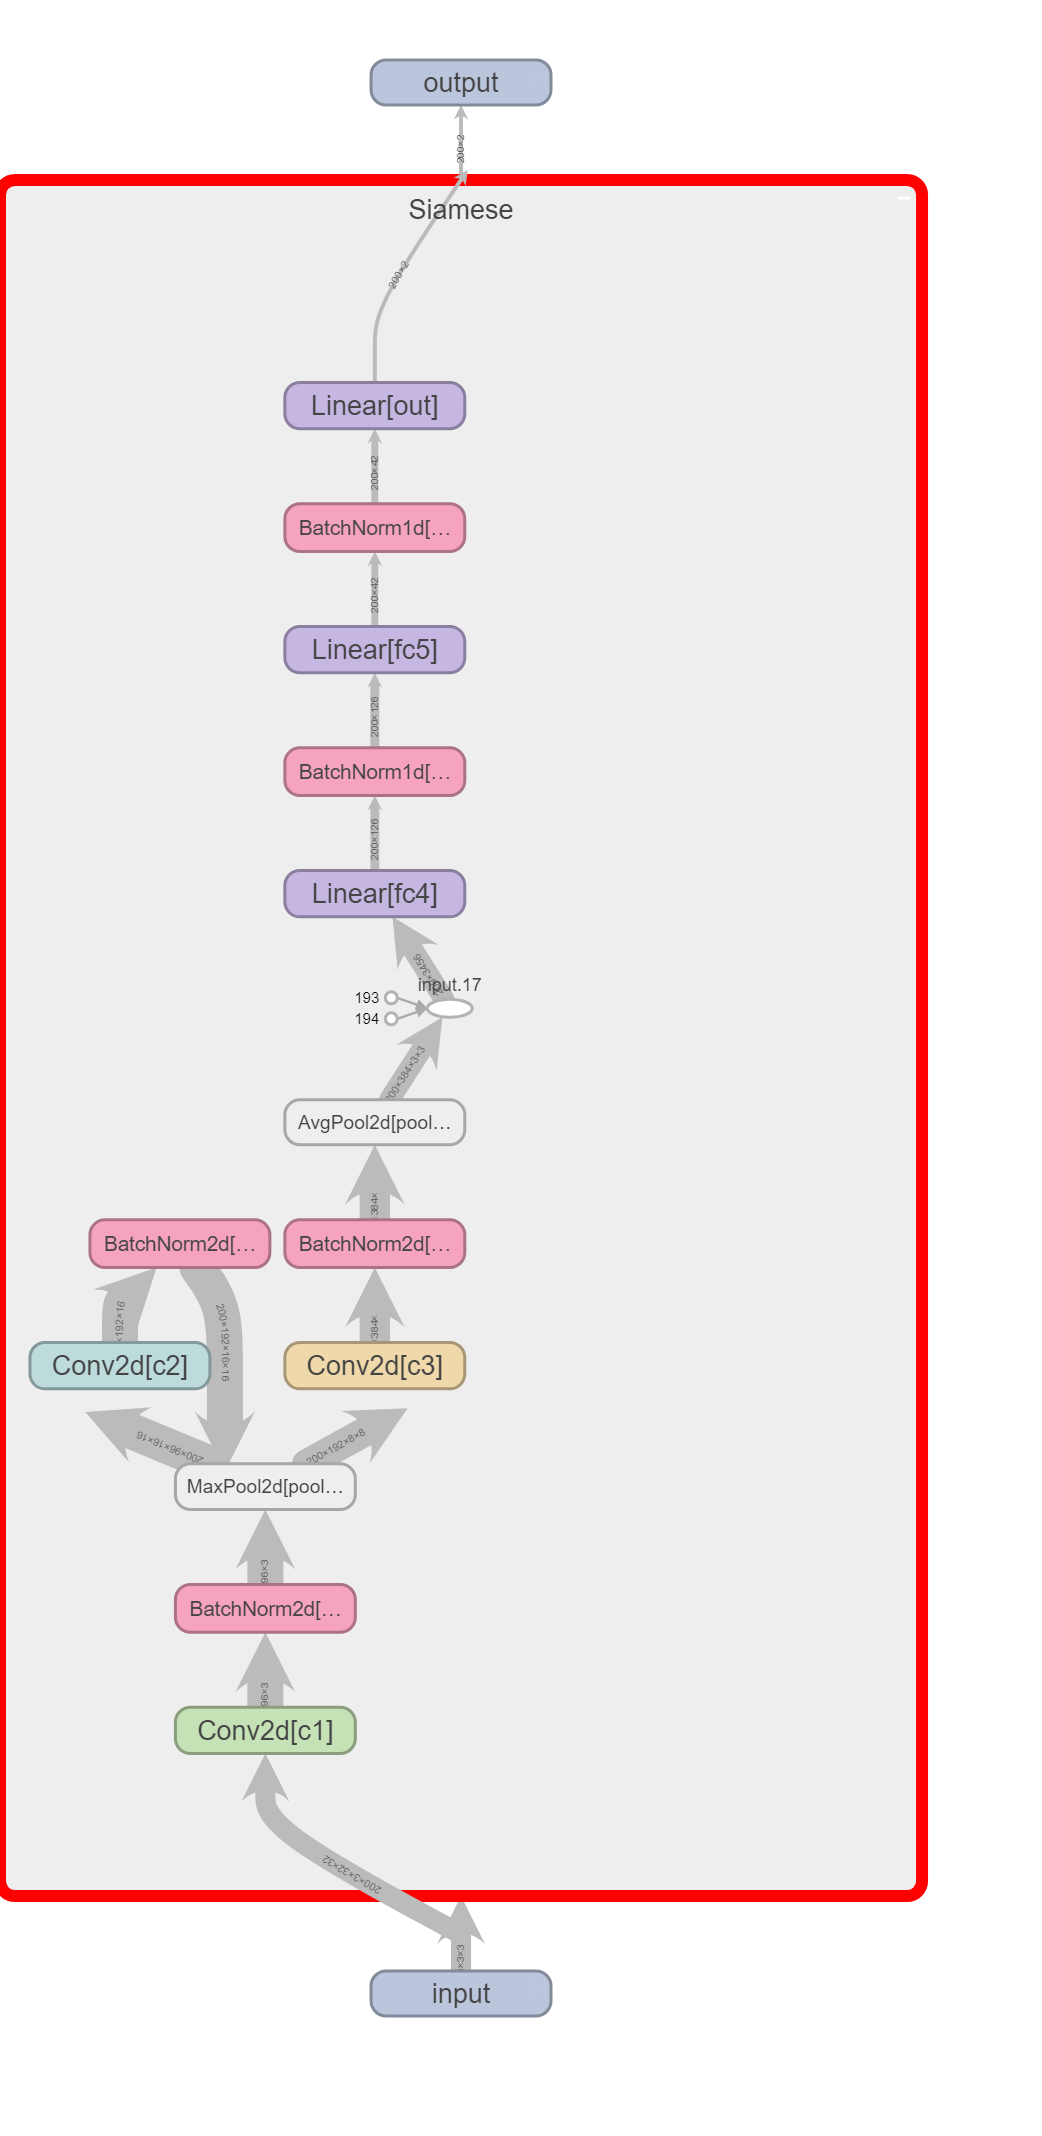
\includegraphics{report_picture/SIA.png} \#\#\# Summary and the
disadvantages This model performs well on the MNIST dataset, and is
relatively easy to train. However, when I apply this model to the CIFAR
dataset, it becomes hard to train and doesn't perform well.
\end{quote}

\hypertarget{reference}{%
\subsubsection{Reference}\label{reference}}

\begin{enumerate}
\def\labelenumi{\arabic{enumi}.}
\tightlist
\item
  Appalaraju S, Chaoji V. Image similarity using deep CNN and curriculum
  learning{[}J{]}. arXiv preprint arXiv:1709.08761, 2017.
\item
  \href{https://en.wikipedia.org/wiki/Siamese_neural_network}{Siamese
  neural network}
\item
  Utkin L, Kovalev M, Kasimov E. An explanation method for Siamese
  neural networks{[}C{]}//Proceedings of International Scientific
  Conference on Telecommunications, Computing and Control. Springer,
  Singapore, 2021: 219-230.
\end{enumerate}

\hypertarget{code-and-result}{%
\subsubsection{Code and result}\label{code-and-result}}

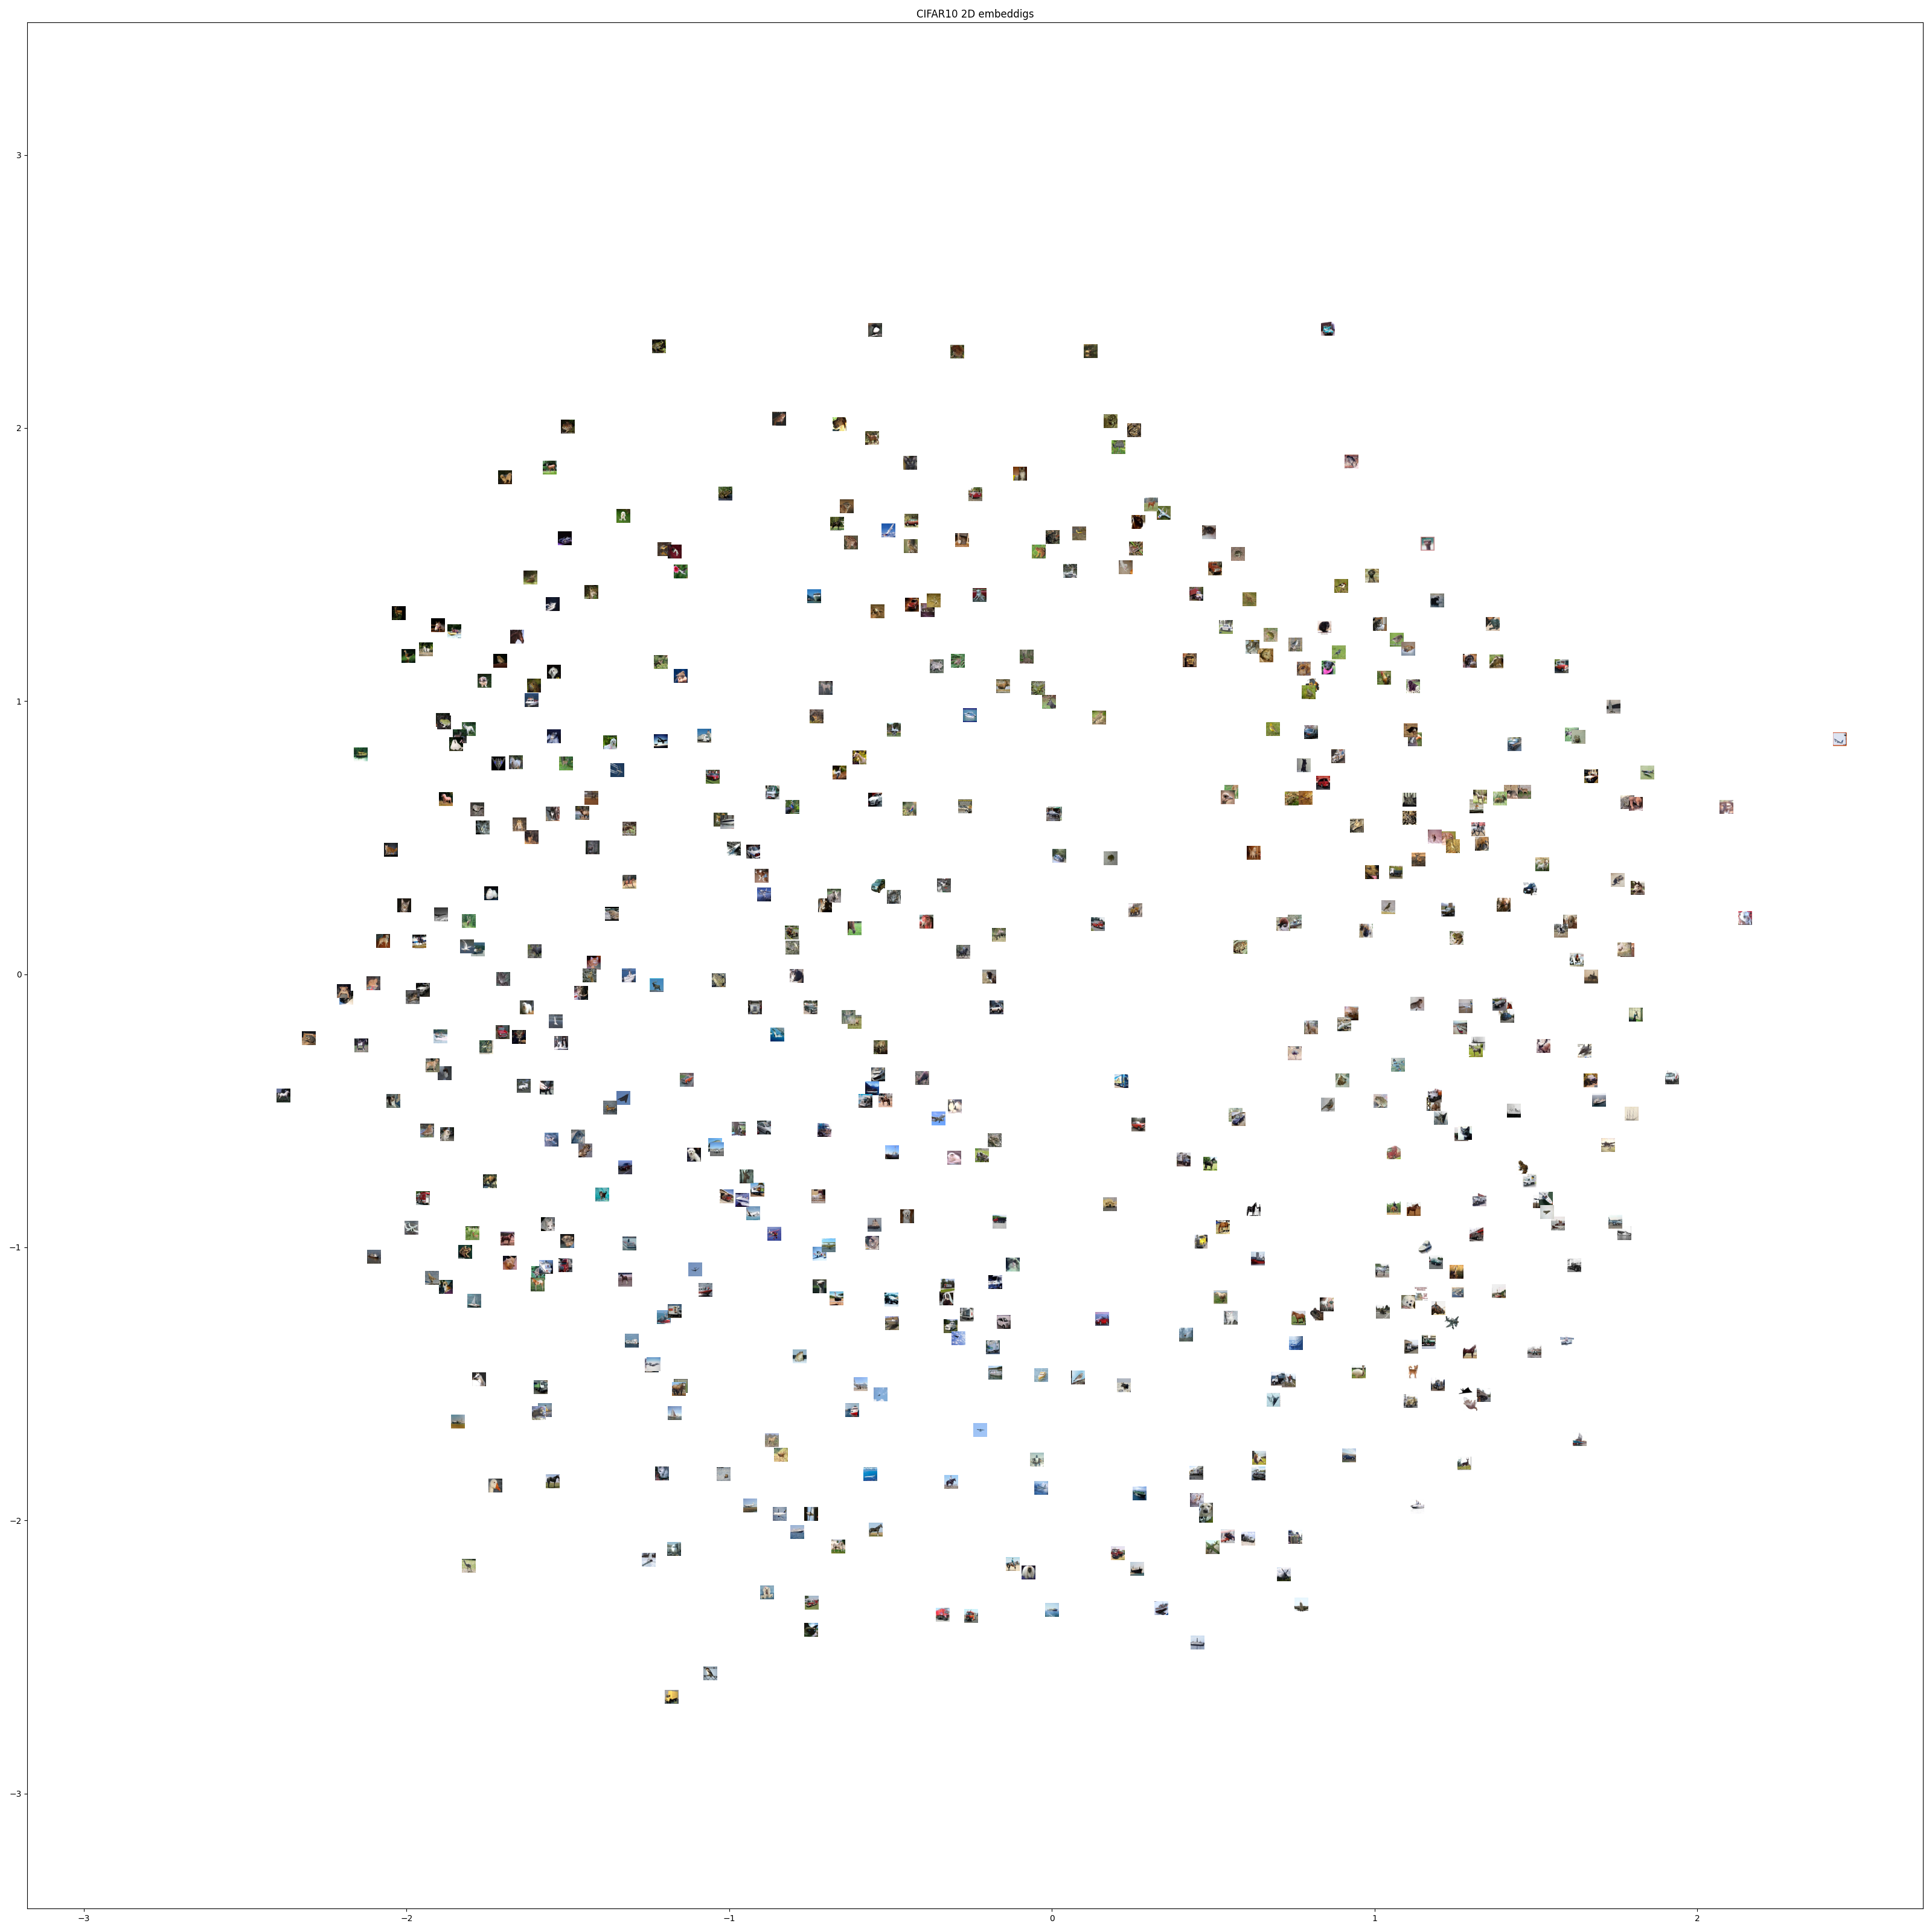
\includegraphics{distribution.png} 
\includegraphics{task2_ans.png}

    \hypertarget{b1reconstruct-images-from-cifar-or-mnist}{%
\subsection{{[}B1{]}Reconstruct images from CIFAR or
MNIST}\label{b1reconstruct-images-from-cifar-or-mnist}}

\hypertarget{introduction-and-my-personal-ideal-towards-this-task}{%
\subsubsection{Introduction and my personal ideal towards this
task}\label{introduction-and-my-personal-ideal-towards-this-task}}

In this task, I need to reconstruct a image from CIFAR or from MNIST.
First I tried a VAE autoencoder. It has the ability to reconstruct the
picture from the latent space, and is pretty easy to train on the MNIST
dataset. However, it cannot reconstruct the image from an noisy image.
\textgreater{}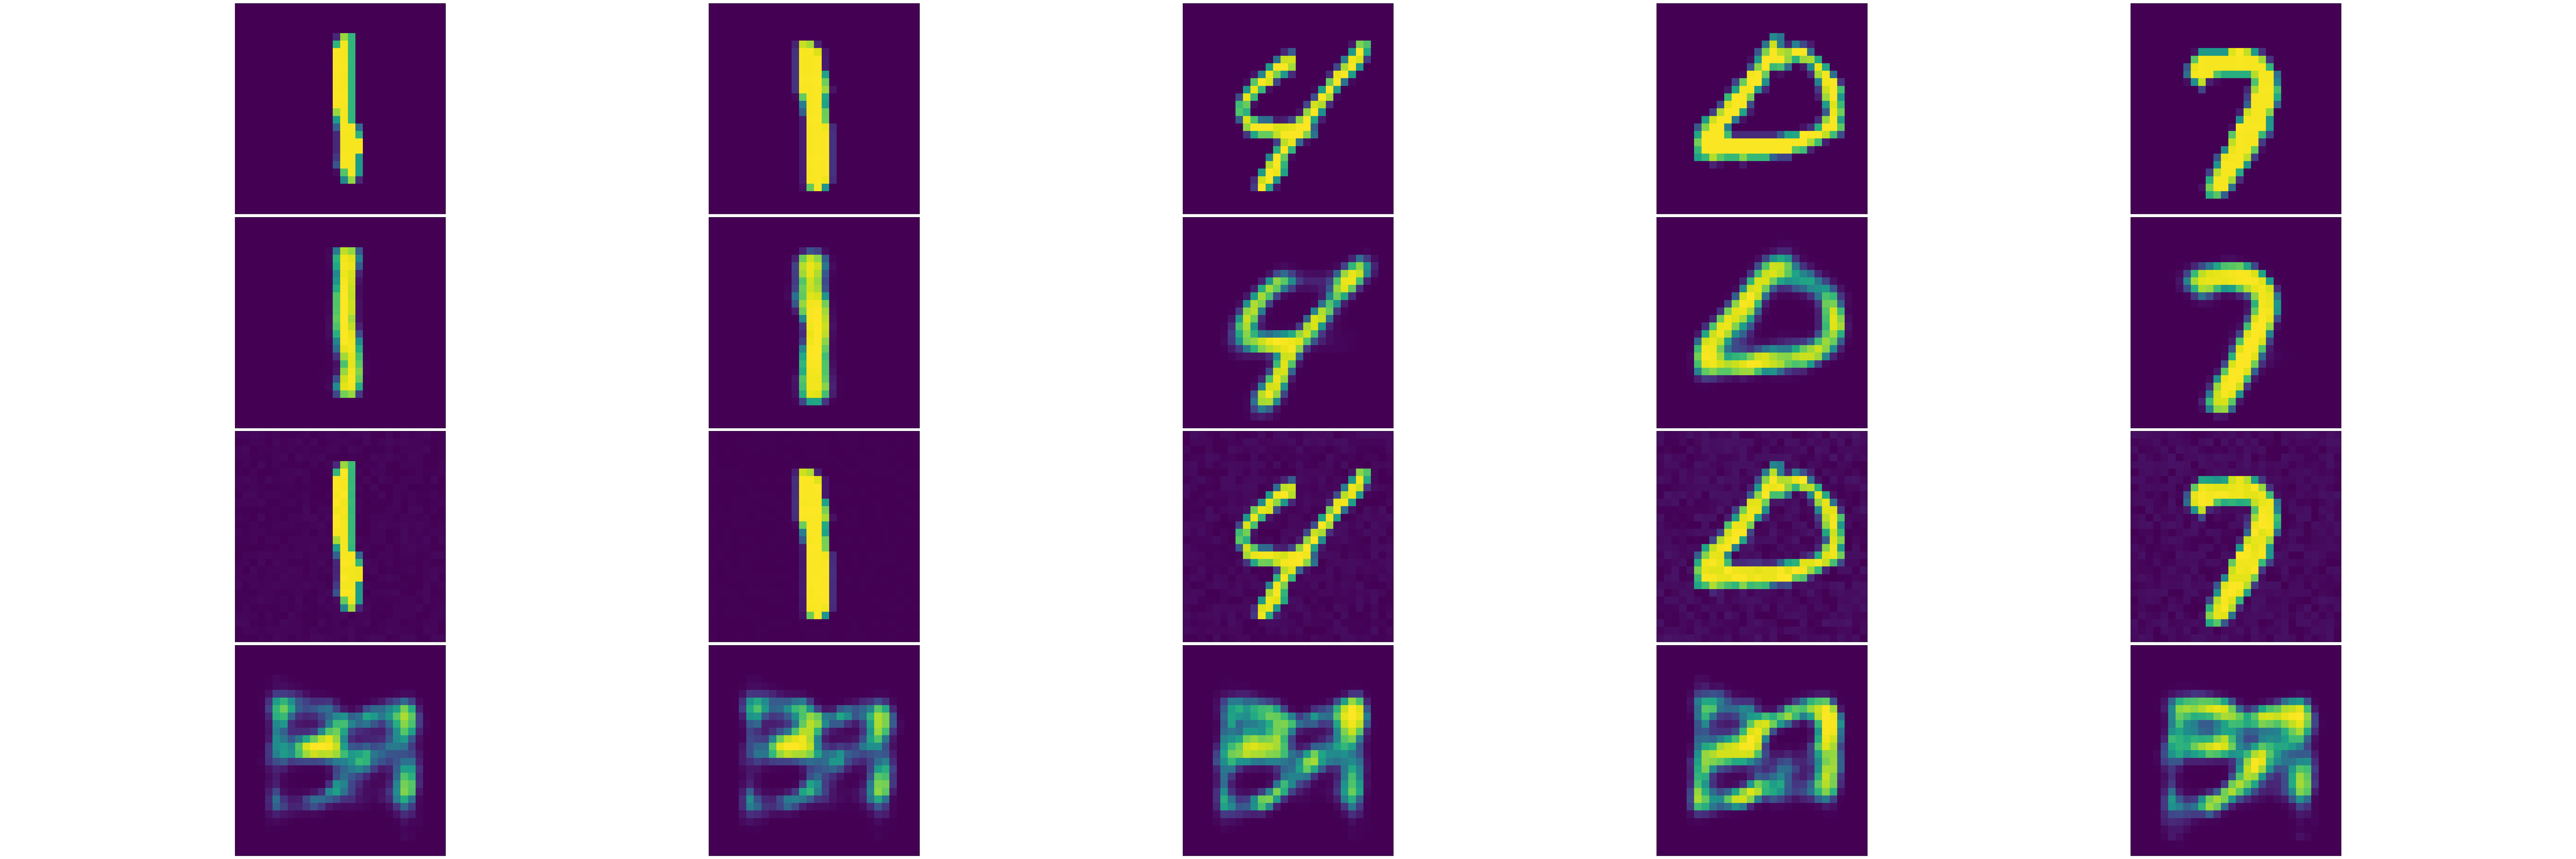
\includegraphics{VAE_ans_20.png} FIG\_1: First line of
pictures are the origin pictures, the second line of pictures are the
images which reconstructed by VAE from the origin pictures, the third
line of the pictures are the noisy version of the origin pictures, the
final line of the pictures are the images which reconstructed by VAE
from the noisy pictures.

Fig1 shows VAE network cannot handle the noisy input pictures. Because
the VAE is tried to memorize the images in the dataset, and a noisy
image does not belongs to the dataset. The VAE is try to use the encoder
find the points in the latent space which represent the images in the
dataset, then use the decoder to reconstruct, so when giving it a image
doesn't belongs to the training dataset, it cannot find the proper point
in the latent space, thus cannot use the decoder to reconstruct the
image. May be a lossy encoding can solve the problem by ignoring the
noise in the image, but my VAE didn't solve the problem.

After realized the VAE network cannot performs well on this task, I
thought may be the diffusion model can solve this problem.
\textgreater\#\#\#\# A brief introduction to the Diffusion model
Diffusion model is a model that not reconstruct the picture in just one
time but several times instead, each time it removes a little bit of
noise in the image, after running plenty of times, it can remove all the
noise in the image. If the input is a pure noisy image, it can generate
a new picture from the input which belongs to the dataset.

By consider the input noisy image as a image in the middle of the pure
noisy and the input image, we can use the diffusion progress to remove
the noise in the input image and reconstruct the image. Here are some of
the result \textgreater{}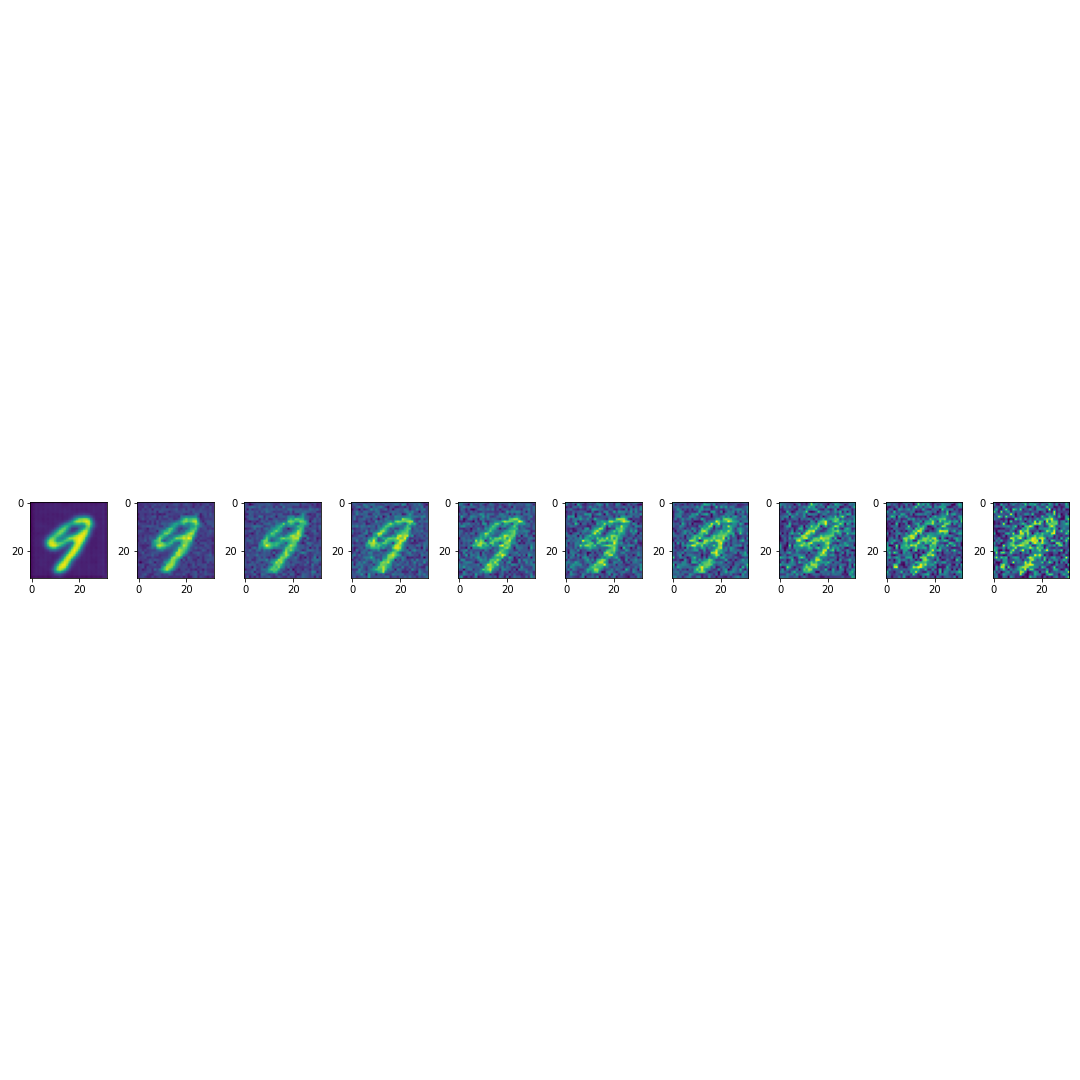
\includegraphics{diffusion_result/0.png}
FIG\_2: the picture on the right is the input noisy image, and the
picture on the left is the result diffusion model gives.

\hypertarget{diffusion-model-explaination-from-httpsen.wikipedia.orgwikidiffusion_model}{%
\subsubsection{Diffusion model (explaination from
https://en.wikipedia.org/wiki/Diffusion\_model)}\label{diffusion-model-explaination-from-httpsen.wikipedia.orgwikidiffusion_model}}

In machine learning, diffusion models, also known as diffusion
probabilistic models or score-based generative models, are a class of
latent variable generative models. A diffusion model consists of three
major components: the forward process, the reverse process, and the
sampling procedure. The goal of diffusion models is to learn a diffusion
process that generates the probability distribution of a given dataset.
They learn the latent structure of a dataset by modeling the way in
which data points diffuse through their latent space.

In the case of computer vision, diffusion models can be applied to a
variety of tasks, including image denoising, inpainting,
super-resolution, and image generation. This typically involves training
a neural network to sequentially denoise images blurred with Gaussian
noise. The model is trained to reverse the process of adding noise to an
image. After training to convergence, it can be used for image
generation by starting with an image composed of random noise for the
network to iteratively denoise. Announced on 13 April 2022, OpenAI's
text-to-image model DALL-E 2 is an example that uses diffusion models
for both the model's prior (which produces an image embedding given a
text caption) and the decoder that generates the final image. Diffusion
models have recently found applications in natural language processing
(NLP), particularly in areas like text generation and summarization.

Diffusion models are typically formulated as markov chains and trained
using variational inference. Examples of generic diffusion modeling
frameworks used in computer vision are denoising diffusion probabilistic
models, noise conditioned score networks, and stochastic differential
equations.

\hypertarget{my-personal-understanding-towards-diffusion-model-and-the-modification-for-the-task}{%
\subsubsection{My personal understanding towards Diffusion model and the
modification for the
task}\label{my-personal-understanding-towards-diffusion-model-and-the-modification-for-the-task}}

In diffusion model we consider the noise image is generated by a
noisyless picture through a markov chain, which gives us a chance to
remove the noise through a opposite progress. The markov chain also
gives us a chance to not to insert the noise many times in order to turn
a image to a noise image, instead the markov chain provide a
mathematical proof to generate the noise image in one time. Here I'm not
going to give a mathiematical proof here, because I don't think I can
explain better than this paper ``Denoising Diffusion Probabilistic
Models'' So what we do in the training progress of diffusion model is
that generating a \(T\) level noisy image and then send it to the U-net
to get a predicted noise distribute. Then use the loss function to judge
the distance of the noise added and the predicted noise. When we need to
reconstruct the image, we need to inverse the Markov chain, and after
minus the predicted noise in each step, we need to add another standard
normal distribution noise to the image in order to get the result. The
paper didn't explain why they need add back this noise, so I guess that
this noise is try to bring the wrongly predicted pixes back to noise. So
in this way, we can generate a image from a pure noise image, but also
with a little modify, we can denoise the picture, by just simply change
the start point of the denoise progress. In this task I used a simple
U-net and without using the VAE encoder and decoder, because I think the
\(1*32*32\) image is relatively small, I don't think using a complex
U-net and the VAE encoder and decoder can largly improve the performance
of the model, on the contrary, I think that make a complex model may
cause overfitting problem and will largly increase the cost of time. I
also want to use another simple cnn net to predict how much rounds of
noise is insert in the picture, however the cnn network doesn't accuracy
enough so I just simply mannuly input the predict of the noise rounds.
\#\#\# My network structure My Simple U-net network structure is look
like the graph below.

\begin{quote}
\begin{figure}
\centering
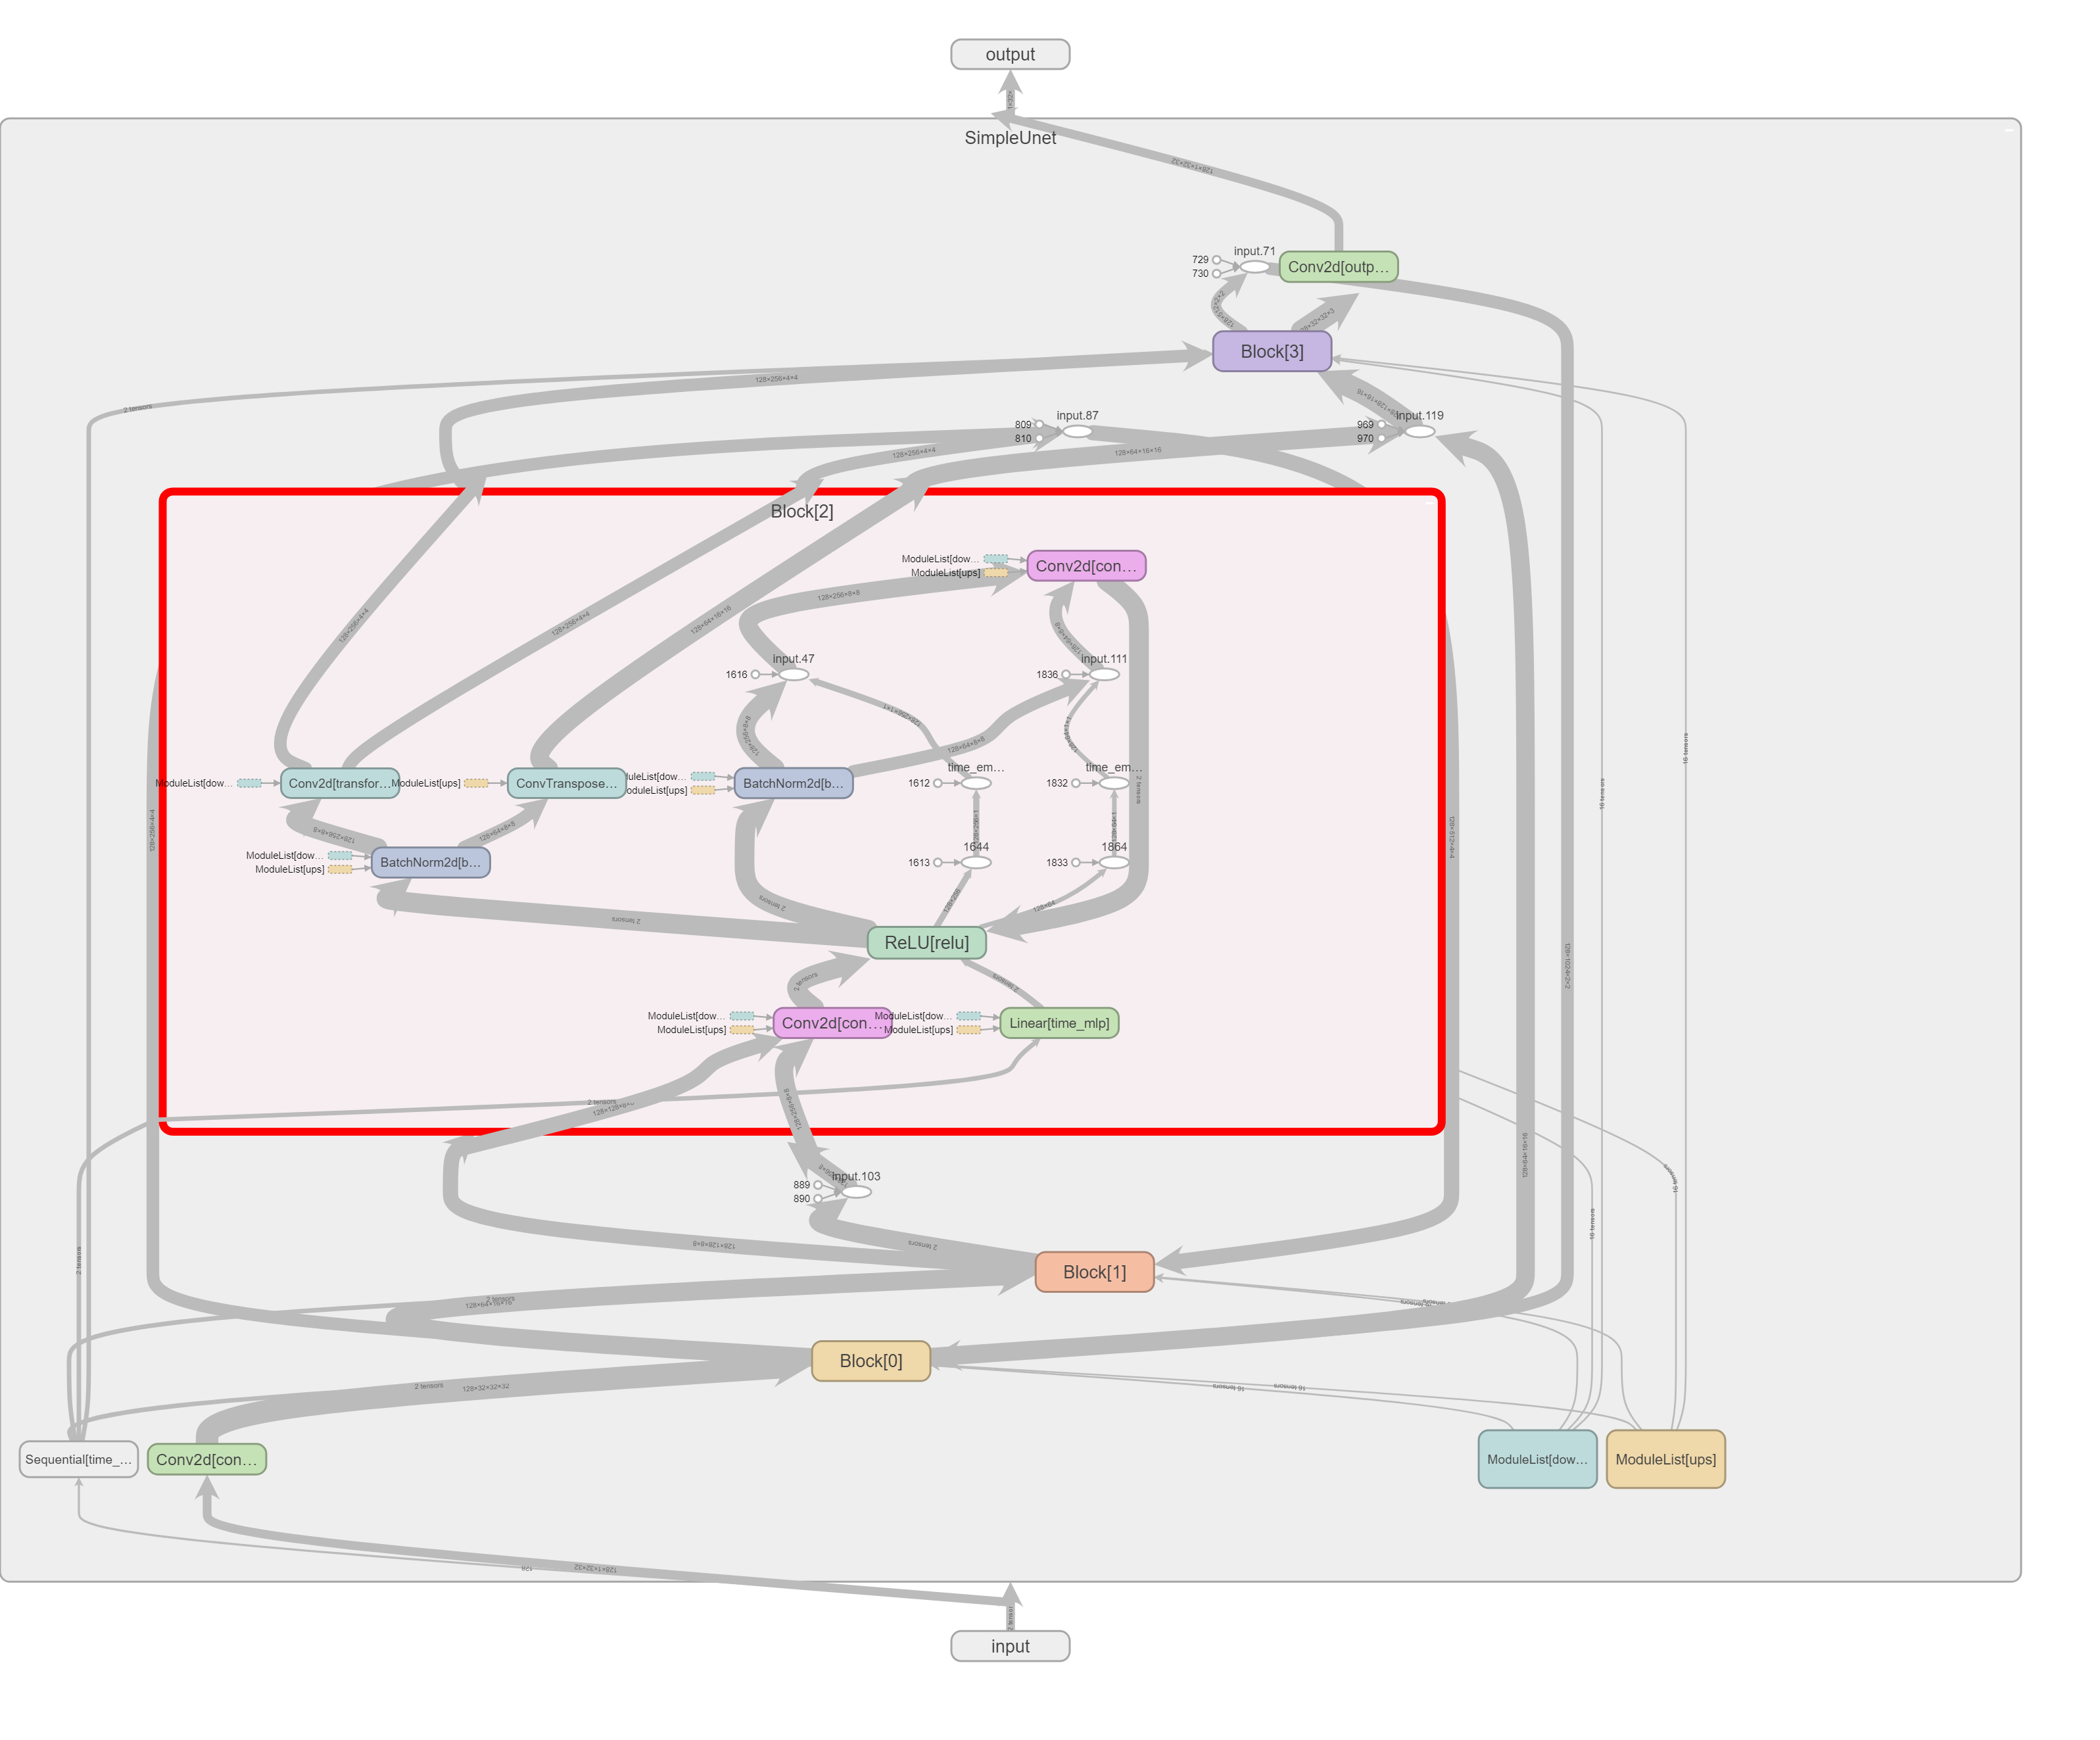
\includegraphics{report_picture/DIFF.png}
\caption{Unet structure}
\end{figure}
\end{quote}

\hypertarget{summary-and-the-disadvantages}{%
\subsubsection{Summary and the
disadvantages}\label{summary-and-the-disadvantages}}

It works well on the MNISt dataset, it can clear the noise I add into
the original image. The model can turn the noisy image into a sharp and
clear image. However this model is still a generative model, so
sometimes its result doesn't look like the original image. such as
sometimes it will turn a noisy ``8'' image into ``6''. May be adding the
text guide into the model will have a better performance.

\hypertarget{code-and-result}{%
\subsubsection{Code and result}\label{code-and-result}}

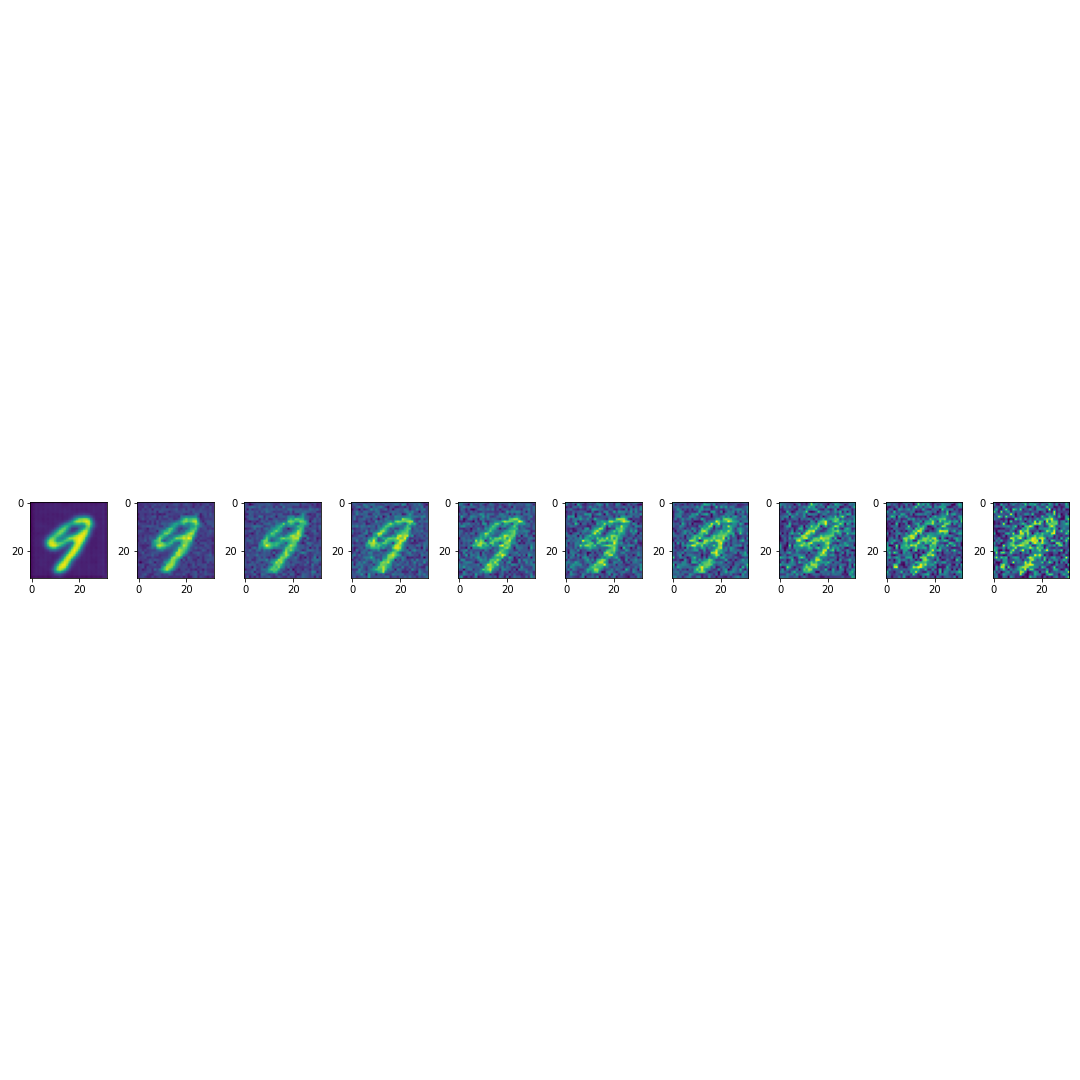
\includegraphics{diffusion_result/0.png}

\includegraphics{diffusion_result/2.png}
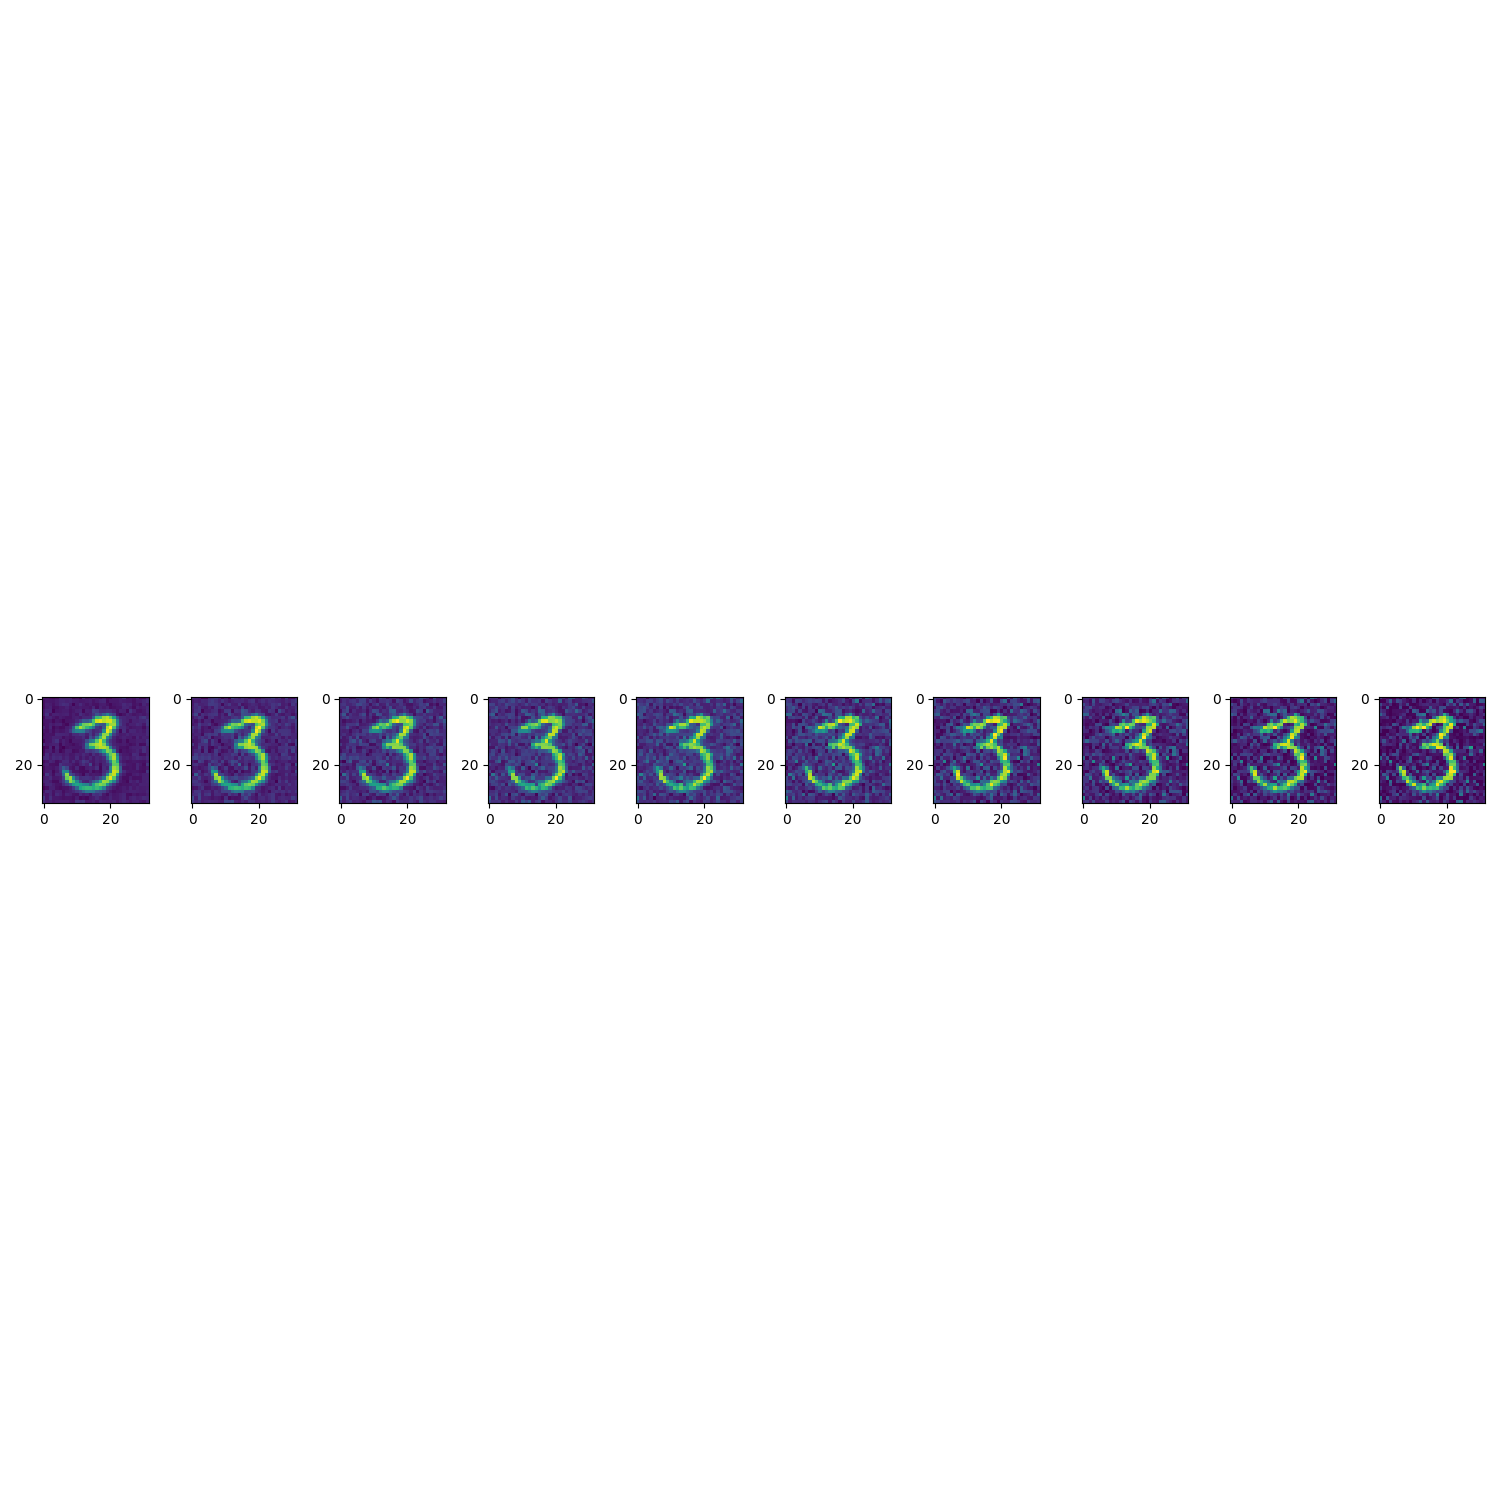
\includegraphics{diffusion_result/9.png}

\includegraphics{diffusion_result/6.png}
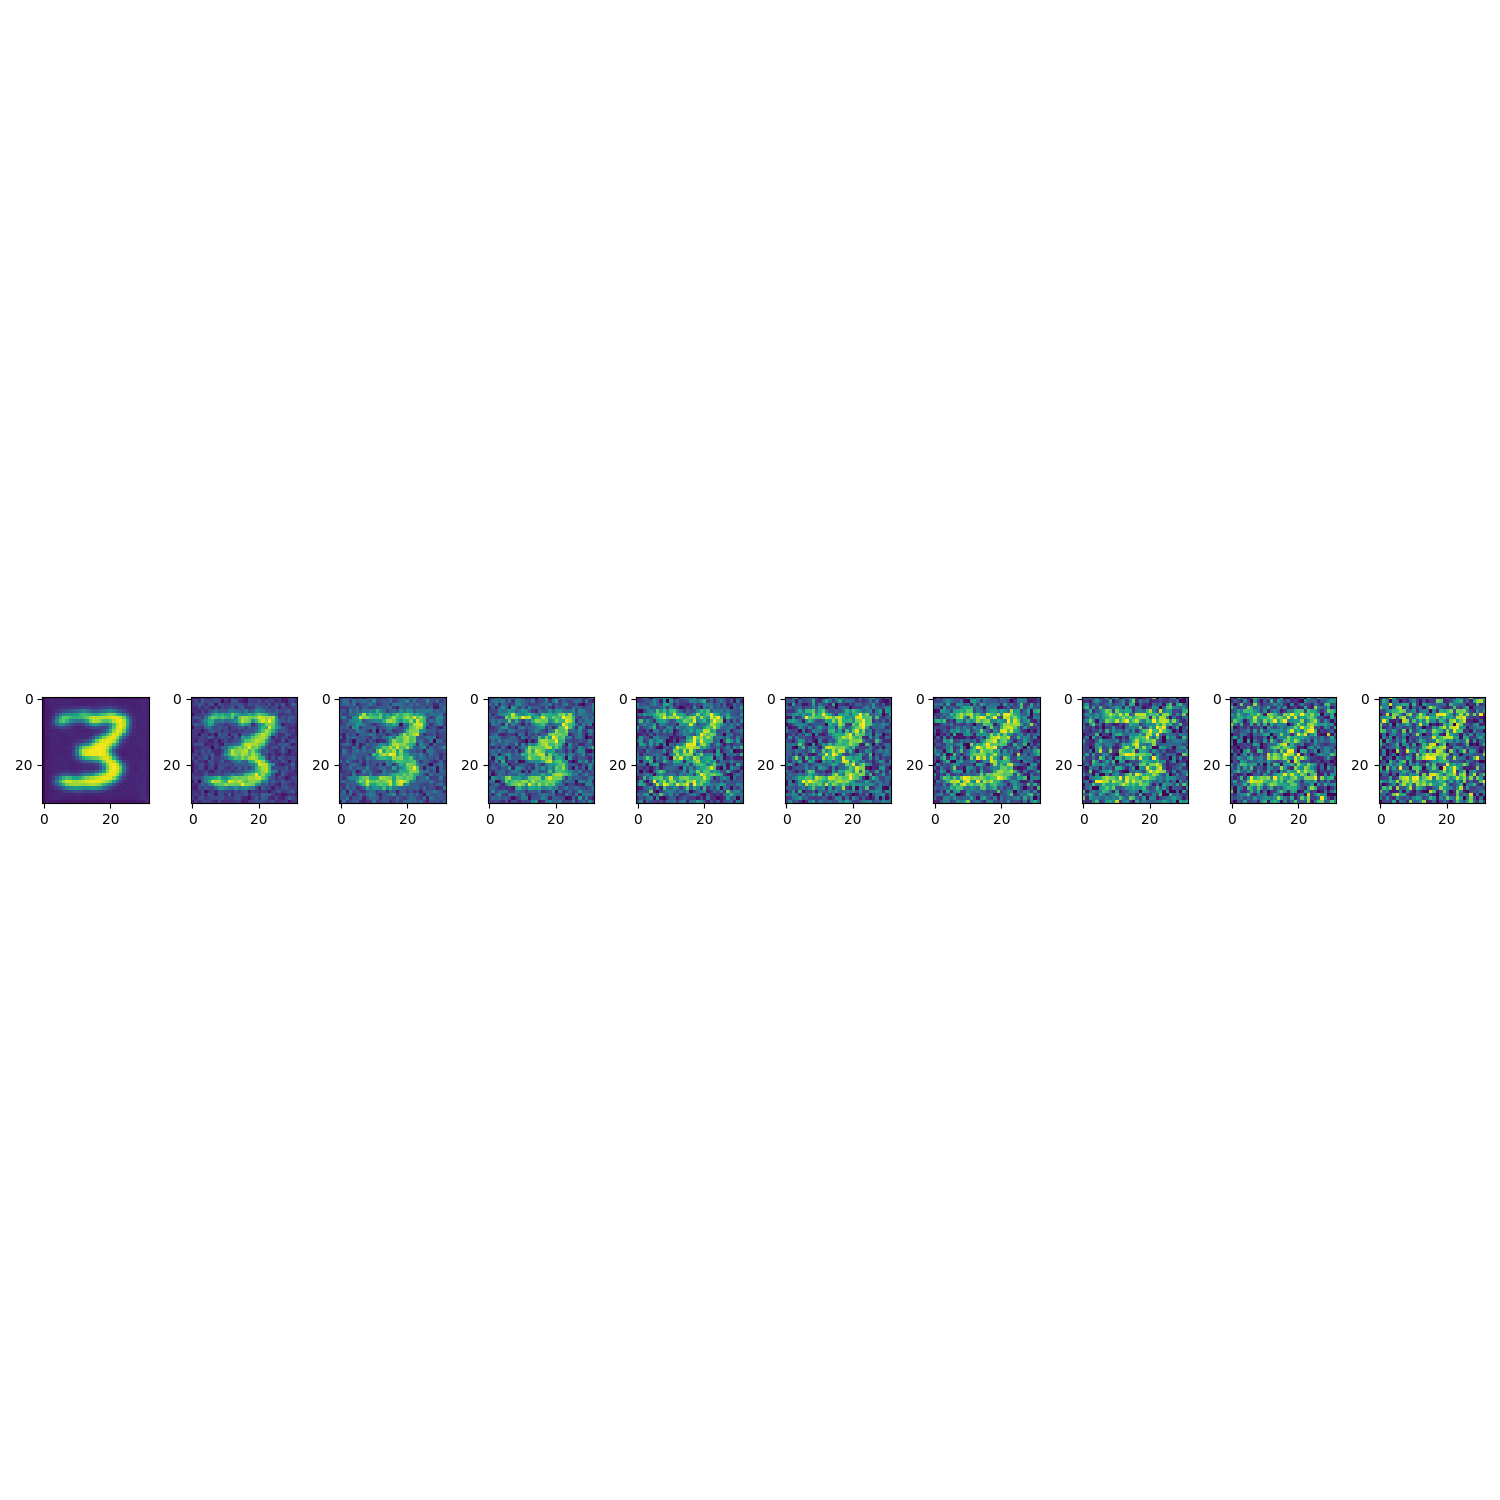
\includegraphics{diffusion_result/8.png}

    \begin{tcolorbox}[breakable, size=fbox, boxrule=1pt, pad at break*=1mm,colback=cellbackground, colframe=cellborder]
\prompt{In}{incolor}{ }{\boxspacing}
\begin{Verbatim}[commandchars=\\\{\}]

\end{Verbatim}
\end{tcolorbox}

    \begin{tcolorbox}[breakable, size=fbox, boxrule=1pt, pad at break*=1mm,colback=cellbackground, colframe=cellborder]
\prompt{In}{incolor}{ }{\boxspacing}
\begin{Verbatim}[commandchars=\\\{\}]

\end{Verbatim}
\end{tcolorbox}


    % Add a bibliography block to the postdoc
    
    
    
\end{document}
